% DoseRAD2026 final submission — Task: PHOTON-CT (single-task LNCS report, <=11 content pages).
% Derived from paper_LNCS_v1.tex (4-task version); task-focused expansion.
\documentclass{llncs}
\usepackage{amsmath,amssymb,bm,mathtools}
\usepackage{graphicx,booktabs,array}
\usepackage[hidelinks]{hyperref}
\usepackage{tikz}
\usetikzlibrary{arrows.meta,positioning,fit,backgrounds}
\graphicspath{{figs/}}
\newcommand{\opS}{\mathcal{S}}\newcommand{\opD}{\mathcal{D}}\newcommand{\opX}{\mathcal{X}}
\newcommand{\opR}{\mathcal{R}}\newcommand{\opC}{\mathcal{C}}\newcommand{\gam}{\gamma}
\renewcommand{\topfraction}{.95}\renewcommand{\bottomfraction}{.6}
\renewcommand{\textfraction}{.05}\renewcommand{\floatpagefraction}{.75}
\setcounter{topnumber}{3}\setcounter{totalnumber}{5}

\begin{document}

\title{A Differentiable Physics-Prior Residual 3D U-Net for Control-Point-Level Photon Dose
Prediction on CT (DoseRAD2026 Photon-CT Task)}
\titlerunning{Physics-Prior Residual U-Net for Photon-CT}
\author{Kai Wang \and Meixu Chen \and Rui Yang}
\authorrunning{K. Wang et al.}
\institute{Department of Radiation Oncology, University of Colorado Anschutz Medical Campus,
Aurora, CO, USA\\ \email{\{kai.2.wang,meixu.chen,ray.yang\}@cuanschutz.edu}}

\maketitle

\begin{abstract}
We predict the Monte-Carlo (MC) dose of every photon MLC control point with an analytical,
differentiable physics prior followed by a residual 3D U-Net. Six channels (density,
radiological depth, primary fluence, distance-to-CAX, source distance, and a naive analytical
dose surrogate are computed per control point from the CT density and the beam descriptor; a
3D U-Net (dilated bottleneck, Softplus head) learns only the residual to MC. Because the aperture
enters as a fluence \emph{input}, the model is robust to the benchmark's deliberate shift from
random training apertures to clinical VMAT test apertures. In ablation, the analytical prior
contributes $+1.9\,\gam$(1\%/1\,mm) and hard-region loss weighting $+2.8$, stacking to $+4.0$;
multi-modal joint training across real- and synthetic-CT inputs adds a further $+2.8$
(cross-validated, every fold). Under 5-fold cross-validation on the 75 public patients the model
reaches plan $\gam$1\%/1\,mm of $93.4\pm1.0$ (multi-modal variant $96.2\pm1.1$). The final
submission is trained on all 75 patients and deployed as a knowledge-distilled base-32 student
(2.1$\times$ faster, \emph{above} the teacher's held-out gamma) with aperture-bbox cropping,
GPU-resident channel construction, compiled inference and cutoff-zeroed output: on the hidden
preliminary test set it scored $\gam$\,=\,95.33, per-beam MAE 0.0107, IDD 0.0072, stratified MAE
0.0049, DVH 0.30 at 80.3\,s per job, well within the 181\,s gate.
\keywords{photon dose prediction \and differentiable physics \and residual learning \and
knowledge distillation \and VMAT}
\end{abstract}

\section{Introduction}
Fast, accurate photon dose calculation underpins online adaptive radiotherapy: a plan must be
recomputed on the anatomy of the day within minutes, at Monte-Carlo (MC)-level accuracy. Deep
dose engines approach this~\cite{photonunet,dota}, but most treat transport as an implicit target
the network must memorize end-to-end. We instead factor the problem: an analytical,
\emph{differentiable} physics operator $\opC$ maps the CT density and the control-point
descriptor to dose-shaped input channels, and a light 3D U-Net $\opD_\theta$ learns only the
residual between this prior and MC. The factorization has three measured consequences. It
reduces learning to a smooth, bounded correction, so a light network trains stably; it makes the
density-dependence explicit (the same operator powers our MRI-task synthesis training); and it
is what makes the model robust to the benchmark's deliberate aperture shift; training beams are
\emph{random} MLC apertures while test beams are \emph{real clinical VMAT} apertures, and because
the aperture is consumed as a fluence input rather than memorized, this shift is absorbed by
construction. This report details the Photon-CT system; the same framework (shared architecture,
different channels) serves our submissions to all four DoseRAD2026 tasks.

\begin{figure}[t]\centering
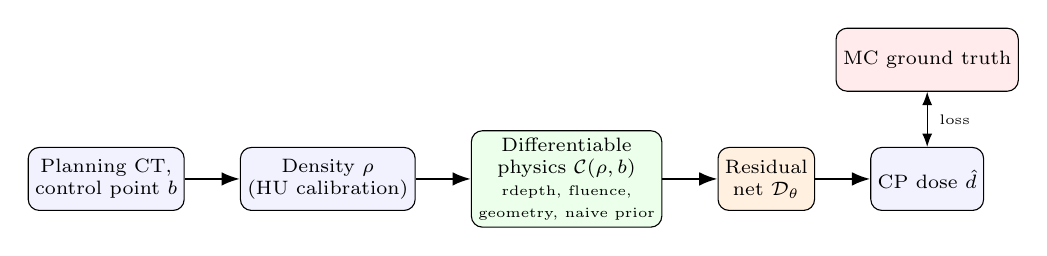
\begin{tikzpicture}[
 node distance=6mm and 7mm, >=Latex, font=\scriptsize,
 box/.style={draw, rounded corners, align=center, minimum height=8mm, inner sep=2.5pt, fill=blue!5},
 phys/.style={box, fill=green!8}, net/.style={box, fill=orange!12},
 every edge/.style={draw, ->, thick}]
\node[box] (img) {Planning CT,\\ control point $b$};
\node[box, right=of img] (dens) {Density $\rho$\\ (HU calibration)};
\node[phys, right=of dens] (chan) {Differentiable\\ physics $\opC(\rho,b)$\\ \tiny rdepth, fluence,\\ \tiny geometry, naive prior};
\node[net, right=of chan] (net) {Residual\\ net $\opD_\theta$};
\node[box, right=of net] (dose) {CP dose $\hat d$};
\node[box, above=7mm of dose, fill=red!8] (mc) {MC ground truth};
\draw (img) edge (dens) (dens) edge (chan) (chan) edge (net) (net) edge (dose);
\draw[<->] (dose) -- (mc) node[midway,right=1pt]{\tiny loss};
\end{tikzpicture}
\caption{Photon-CT pipeline: per control point, differentiable physics channels from the CT
density; a 3D U-Net corrects the analytical prior toward MC.}\label{fig:framework}
\end{figure}

\begin{figure}[t]\centering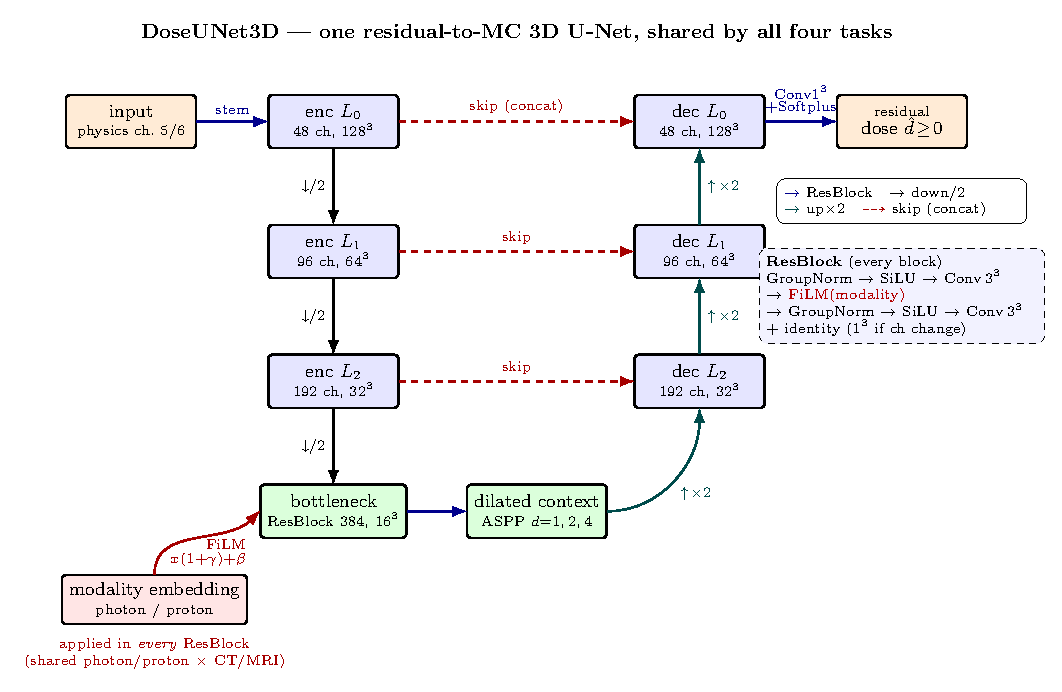
\includegraphics[width=.78\linewidth]{model_arch.pdf}
\caption{The dose network $\opD_\theta$ (DoseUNet3D): residual-to-MC 3D U-Net (channels
48/96/192/384; the deployed distilled student uses base 32), strided-conv down / transpose-conv
up, dilated-context (ASPP, $d{=}1,2,4$) bottleneck for long-range lateral scatter, Softplus head
(non-negative dose), FiLM modality conditioning in every ResBlock.}\label{fig:arch}\end{figure}

\section{Methods}
\subsection{Data}
We use only the official DoseRAD2026 training set~\cite{challenge} (75 patients: 39 thorax, 36
abdomen), built on the SynthRAD2025 cohort~\cite{synthrad}: per patient a planning CT, beam
parameters, and per-control-point Monte-Carlo dose-to-medium in absolute Gy (Geant4 full particle transport; the VMAT plans themselves are generated with matRad~\cite{matrad}) on a
$2{\times}2{\times}2$\,mm grid; 540 control points per patient. Training apertures are random;
test apertures are real clinical VMAT (a deliberate distribution shift, Sec.~1). No external
data are used for this task. For development we ran 5-fold cross-validation (CV) over all 75
patients (every patient held out exactly once); \textbf{the final submitted model is retrained
on all 75 patients}, with the challenge leaderboard as the held-out validation signal.

\subsection{Model}
$\hat d=\opD_\theta(\opC(\rho,b))$, with $\rho$ from the official piecewise-linear
HU$\to$density calibration. The operator $\opC$ assembles \textbf{six channels} per control
point, all implemented as differentiable tensor operations:
(1) \emph{density} $\rho$;
(2) \emph{radiological depth}, the line integral $\int\rho\,d\ell$ from source to voxel,
ray-marched along divergent rays with trilinear sampling; the water-equivalent depth that
drives primary attenuation and build-up;
(3) \emph{primary fluence}: the MLC/jaw aperture of the control point projected through the
divergent beam geometry onto each voxel and attenuated by $\exp(-\mu\,\mathrm{rdepth})$ with a
6\,MV effective coefficient;
(4) \emph{distance to the central axis} (penumbra and off-axis softening);
(5) \emph{source distance} (inverse-square fall-off);
(6) a \emph{naive analytical dose surrogate}
(fluence $\times$ inverse-square $\times$ build-up), a smooth, physically grounded starting
estimate the network corrects.
A per-ray \emph{skin-entry} rule governs the depth and prior: along each ray, depth accumulates
only from the first voxel with $\rho>0.05$\,g/cm$^3$, and the prior is masked strictly upstream
of that crossing: no dose before the body, nothing suppressed inside it (internal air cavities
preserved). $\opD_\theta$ is DoseUNet3D (Fig.~\ref{fig:arch}): base 48 (teacher), four levels,
ASPP bottleneck, Softplus head, FiLM conditioning; the \emph{deployed} network is a base-32
student distilled from it (Sec.~2.3). Figure~\ref{fig:chain} visualizes the full
residual-learning chain of the deployed model.

\begin{figure}[t]\centering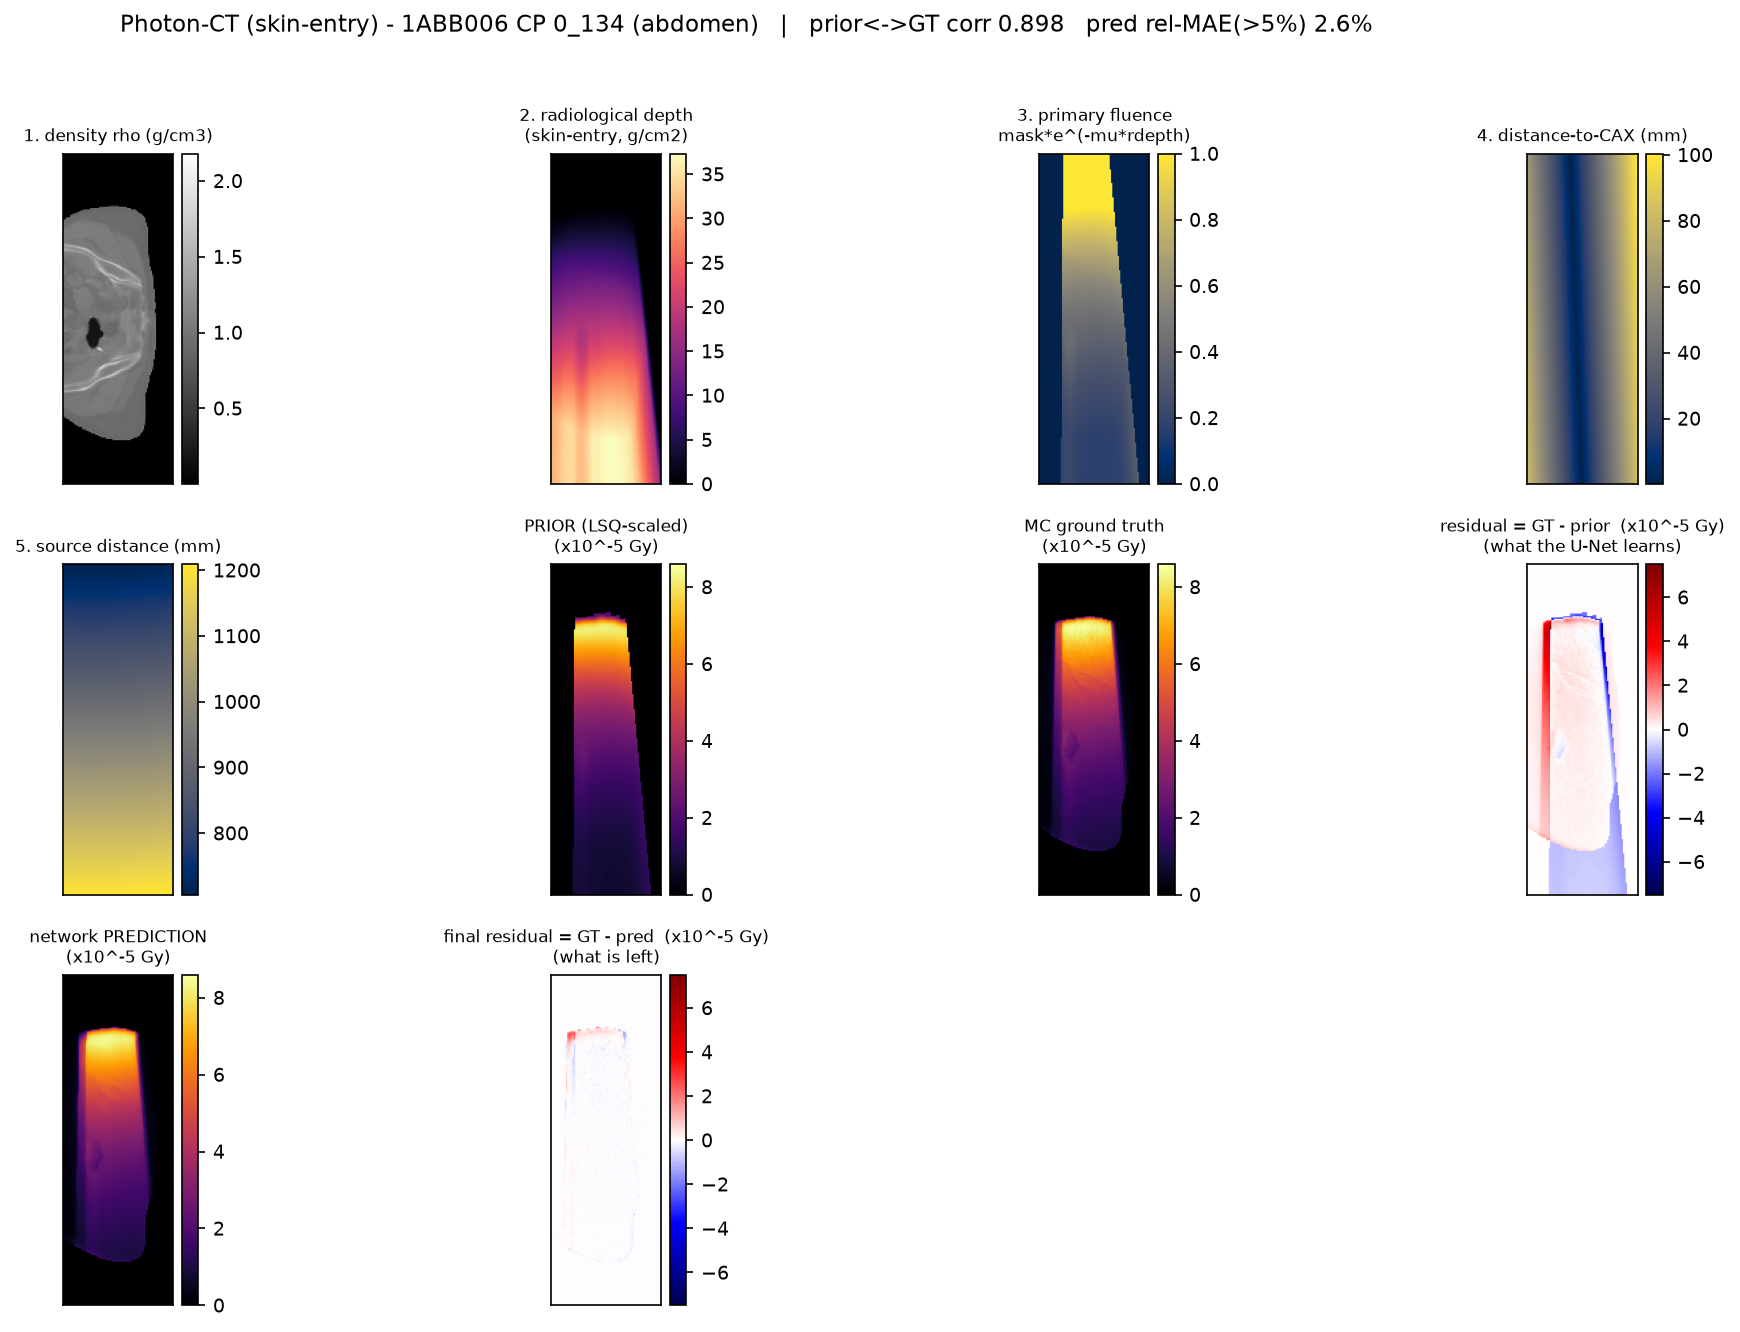
\includegraphics[width=.88\linewidth]{figS_residual_photonct_abdomen.png}
\caption{Residual-learning chain of the deployed skin-entry model (abdomen, 1ABB006, peak-dose
control point): input channels (density, radiological depth, primary fluence, distance-to-CAX,
source distance) $\to$ LSQ-scaled naive prior $\to$ MC ground truth $\to$ residual (GT$-$prior)
$\to$ network prediction $\to$ final residual (GT$-$pred). Both residual panels share one
symmetric window: the shrinkage is the network's contribution.}\label{fig:chain}\end{figure}



\subsection{Training}
Loss: high-dose-weighted $L_1$ to MC (high-dose fraction 0.1, weight 10) plus bounded
penumbra/interface/lung terms; AdamW (lr $10^{-4}$ scratch, $2\times10^{-5}$ finetune), EMA,
gradient clipping; patches $128^3$, batch 2--4. The base-48 teacher trains $\sim$120k steps plus
finetune. Two further stages define the final submission. \textbf{Multi-modal joint training:}
starting from the trained photon-MRI system, the shared dose network continues training on a
50/50 interleave of real-CT cached-channel batches and MRI end-to-end steps; the resulting
single network is a \emph{better} CT engine than the dedicated CT model (Sec.~3.3).
\textbf{Knowledge distillation (deployment):} the base-48 network is distilled into a base-32
student (7.6M vs.\ 17.1M parameters, 2.1$\times$ faster forward) with a two-stage D-recipe:
200k steps of $L_1(\mathrm{GT})+0.5\,L_1(\mathrm{teacher})$, then a 40k GT-only finetune. The
student finished \emph{above} the teacher's held-out gamma ($+0.33$), so the speed is free.
Reproducibility: fixed seeds, YAML-configured runs, EMA checkpoints; code and weights to be
open-sourced (Sec.~6).

\subsection{Evaluation}
Internal: plan-level local $\gam$~\cite{gamma} (pymedphys, 1\%/1\,mm, $\ge$10\% Rx cutoff,
matching the official metric; verified byte-identical against the vendored official evaluation
code), per-beam masked MAE, official IDD and stratified-MAE reimplementations, and a frozen
16-patient held-out cohort gating every deployment change (rule: \emph{a change ships only if it
loses neither accuracy nor speed}). A pitfall we surfaced and corrected: a photon control point
has broad scatter tails ($\sim$4\% of plan energy outside margin-8 crops), and scoring against
equally-cropped ground truth hides the loss entirely (96.2 vs.\ 86.4 against the full-grid GT on
one patient); all crop margins were therefore selected on \emph{full-grid} metrics. Runtime:
the official score is $T=t_{\rm fix}+N\cdot t_{\rm dose\,map}$, gate 181\,s/job, double-weighted
in the ranking; we profile at job scale under the platform memory budget.

\section{Results}
\subsection{Accuracy: cross-validated and hidden-test}
Table~\ref{tab:res} summarizes accuracy and the official hidden-test metrics. Per-fold CV
$\gam$1/1: 94.0/92.4/94.4/94.2/92.1 (mean $93.4\pm1.0$); the multi-modal variant reaches
$96.2\pm1.1$, a $+2.8$ gain holding on every fold. On the fixed development fold ($n=16$):
$\gam$1/1 $=95.7\pm3.8$ (abdomen 97.4, lung 94.0), $\gam$3/3 $=99.8$; per-beam masked MAE
$1.19\pm0.24$\% of the beam maximum. For reference, the challenge's analytical baseline
(pyRadPlan) reaches only $\gam$1/1 $\approx26.9$ on this metric; the residual network's
correction of the analytical prior is essential.

\begin{table}[t]\centering
\caption{Photon-CT results. CV: 5-fold over the 75 public patients. Hidden test: official
metrics of the final full-data submission on the DoseRAD2026 preliminary test set (August 2026).
The runtime gate is 181\,s/job.}\label{tab:res}
\begin{tabular}{@{}lc@{}}\toprule
Metric & Value\\\midrule
CV plan $\gam$1\%/1\,mm (5-fold) & $93.4\pm1.0$ (multi-modal variant $96.2\pm1.1$)\\
Hidden-test per-beam masked MAE & $0.0107\pm0.0014$\\
Hidden-test IDD curve distance & $0.0072\pm0.0040$\\
Hidden-test stratified plan MAE & $0.0049\pm0.0016$\\
Hidden-test plan $\gam$1\%/1\,mm & $95.33\pm1.89$\\
Hidden-test DVH clinical score & $0.30\pm0.14$\\
Hidden-test runtime per job & 80.3\,s (0.12\,s/CP; distilled student $\sim$0.09\,s/CP)\\\bottomrule
\end{tabular}\end{table}

\subsection{Ablations}
The two Photon-CT-specific levers stack (single held-out fold, $n=16$; Table~\ref{tab:abl}):
the naive analytical prior contributes $+1.9\,\gam$ and hard-region loss weighting $+2.8$,
together $+4.0$ over a plain 5-channel U-Net with uniform $L_1$.

\begin{table}[h]\centering
\caption{Photon-CT ablation (plan $\gam$1\%/1\,mm, $n=16$): analytical prior $\times$
hard-region loss weighting.}\label{tab:abl}
\begin{tabular}{@{}lcc@{}}\toprule
 & uniform $L_1$ & hard-region weighting\\\midrule
no prior (5-ch) & 91.7 & 94.5\\
$+$ naive prior (6-ch) & 93.6 & \textbf{95.7}\\\bottomrule
\end{tabular}\end{table}

\subsection{Multi-modal training exploits the photon residual's head-room}
A cross-validated \emph{real-CT ceiling} experiment first located spare capacity: fed the real
CT, the jointly trained photon-\emph{MRI} dose network outperformed the dedicated CT network by
$+2.4$ points ($95.8\pm1.3$ vs.\ $93.4\pm1.0$), verified through the identical cached-channel
pipeline (weights are the only difference). Testing the implied strategy directly, multi-modal
joint training of one network over real- and synthetic-CT inputs raised CV Photon-CT to
$96.2\pm1.1$ ($+2.8$, on every fold) with the MRI task unchanged. The mechanism is coherent with
the residual design: the photon analytical prior is deliberately crude (it omits scatter,
heterogeneity, penumbra), so the residual is large and structured, and exposure to a broader
distribution of density-to-dose mappings acts as a strong, dose-relevant input augmentation. The
identical experiment on the proton tasks; where the pencil-beam prior already supplies
$\sim$95\% of the dose; is flat, a saturation control that locates the exploitable head-room
precisely in the residual to a \emph{weak} prior.

\subsection{The crop margin is an accuracy--runtime knob, and cropped scoring hides its cost}
We quantified a methodological pitfall that affects any cropped evaluation. A photon control point has
broad scatter tails: $\sim$4\% of the plan's energy falls outside margin-8 crops, concentrated
in the 10--20\%-of-max dose band where a \emph{local} 1\% gamma criterion has almost no
tolerance. Scoring a margin-8 model against equally-cropped cached ground truth hid this
entirely; 96.2 apparent vs.\ 86.4 true against the raw full-grid ground truth on one
patient, so every margin decision was re-made on full-grid metrics. Widening the margin needs
no retraining (the network is fully convolutional over analytic channels), and margin trades
directly against runtime: margin 16 costs $+$0.01--0.02\,s/CP over margin 8 but preserves the
tail dose; margins 8 and 12 lost gamma and IDD on the board; a margin-8 \emph{finetune} (network
retrained at the deployed margin) did not recover the gap, showing the loss is physical tail
truncation, not train--deploy mismatch. Margin 16 with cutoff-zeroed output is the deployed
optimum. A related official-metric detail: the challenge's ground truth zeroes dose below the
per-beam cutoff; matching it by zeroing our sub-cutoff outputs was worth $+3\,\gam$ on the
photon board (for protons, quantising rather than zeroing was better), an example of why we
vendored and byte-verified the official evaluation code.

\subsection{Distillation: the student overtakes the teacher}
The deployed network is a base-32 student (7.6M parameters) of the base-48 teacher (17.1M).
Single-stage distillation converges slowly (fold-0 plan $\gam$ vs.\ steps: 77.7 at 40k, 86.9 at
80k, 93.2 at 160k, 94.0 at 200k = teacher parity 94.0), and the full D-recipe adds a 40k GT-only
finetune, after which the full-data student \emph{exceeded} the teacher's held-out gamma by
$+0.33$ at 2.1$\times$ speed. Two scaling observations: a base-24 student (2.6$\times$) fell
measurably short in probes, and cross-domain reuse fails; the CT-trained student loses
$4.1\,\gam$ when stitched behind an MRI front-end whose synthetic-density channels it never saw,
recoverable only by finetuning on synthesis-domain channels. Distillation is thus
domain-specific but, within domain, strictly dominant at this task size.


\begin{figure}[t]\centering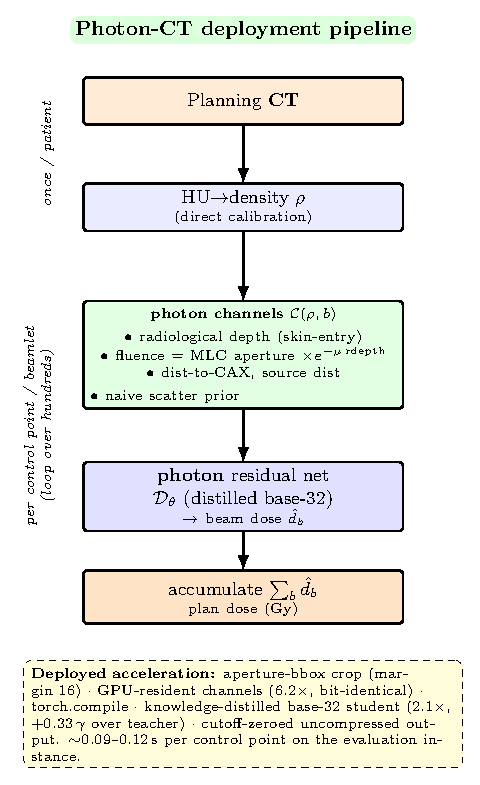
\includegraphics[width=.55\linewidth]{fig_deploy_photonct.pdf}
\caption{The deployed Photon-CT container: per patient, the density stage runs once; the
differentiable-channels $\to$ residual-net loop runs per control point/beamlet. The callout
lists the deployed acceleration measures and their measured effects.}\label{fig:deploy}\end{figure}

\subsection{Runtime engineering}
Runtime is double-weighted, so deployment was treated as a research target under the
no-accuracy-loss gate. Table~\ref{tab:accel} lists the levers. Per control point, an
aperture-derived bounding box (margin 16 voxels, selected on full-grid metrics) crops the
compute domain; all six channels are built GPU-resident ($6.2\times$ over the CPU builder,
bit-identical); the network is compiled (\texttt{torch.compile} pays off here: one grid per
patient, 540 same-shape control points amortize the one-time cost); sub-cutoff outputs are
zeroed and written uncompressed (photon jobs are compute-bound; compression only adds CPU). The
deployed distilled student runs at $\sim$35\,ms/CP on our development GPU and
$\sim$0.09--0.12\,s/CP on the evaluation instance. A negative finding worth reporting: for this
small distilled network, batch-1 inference already saturates the GPU; control-point batching
(1.01--1.09$\times$), asynchronous delayed emission (0.90$\times$), fp16 weights (1.00$\times$)
and autotuned compilation ($-$, platform $t_{\rm fix}$ pays the longer autotune) all failed our
gate; once channel construction and the write path are off the critical path, the convolution
forward itself is the deployment floor.

\begin{table}[t]\centering
\caption{Photon-CT acceleration levers (all accuracy-gated on a frozen held-out cohort;
measured, not estimated).}\label{tab:accel}
\setlength{\tabcolsep}{4pt}\small
\begin{tabular}{@{}lll@{}}\toprule
Lever & Effect & Accuracy impact\\\midrule
Aperture-bbox crop, margin 16 & $-30$\,s/job vs.\ margin 24 & $\gam$ preserved (full-grid gated)\\
GPU-resident channel builder & $6.2\times$ channel build & bit-identical\\
\texttt{torch.compile} (dose net) & $\sim$1.5$\times$ net & exact\\
Distilled base-32 student (D-recipe) & $2.1\times$ net forward & $+0.33\,\gam$ over teacher\\
Zero-cutoff output, no compression & write path off critical path & $+3\,\gam$ (cutoff match)\\
\emph{Rejected:} CP batching / async emission / fp16 & $\le$1.09$\times$ or negative & --- \\\bottomrule
\end{tabular}\end{table}



\begin{figure}[t]\centering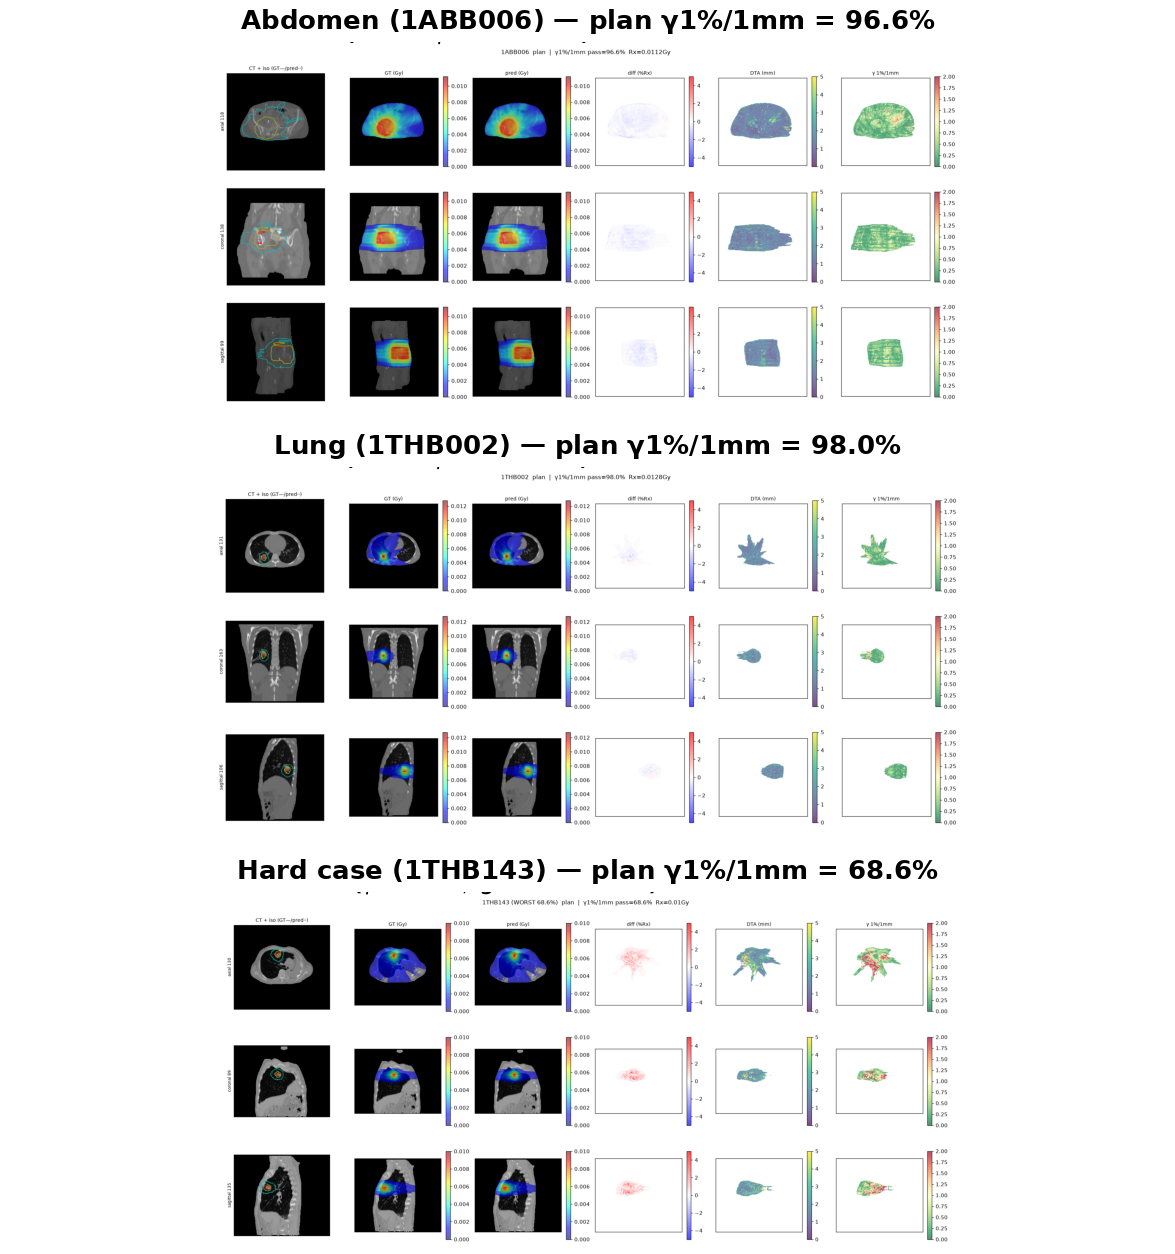
\includegraphics[width=.92\linewidth]{fig_qual_photonct.png}
\caption{Qualitative Photon-CT results on three cases spanning the difficulty range: abdomen (1ABB006, plan $\gam$1/1 $=96.6$), lung (1THB002, $98.0$), and the geometrically hard case 1THB143 ($68.6$; the worst patient in all four challenge tasks simultaneously, yet largely passing at 3\%/3\,mm: small-magnitude errors at steep lung--tissue interfaces). Columns: image with GT (solid) and predicted (dashed) isodose, MC dose, predicted dose, difference, distance-to-agreement, local $\gam$1\%/1\,mm.}\label{fig:qual}\end{figure}

\section{Discussion}
The explicit prior-plus-residual factorization, rather than raw capacity, drives this system's
accuracy, robustness and speed: the ablation shows prior and loss-weighting stack to $+4.0$; the
aperture-as-input design absorbs the random-to-VMAT test shift; and the residual's head-room is
what multi-modal training converts into a further $+2.8$. The deployed model is a distilled
student that is \emph{faster and slightly better} than its teacher, evidence that at this task
size the base-48 network is over-parameterized for the residual it must learn.
\textbf{Limitations and generalizability.} All data come from one benchmark (abdomen/thorax,
single machine model); cross-vendor and cross-site validation is future work. Ablation effects
are single-fold ($n=16$); the headline accuracy is the 5-fold CV. One geometrically hard
thoracic case (large heterogeneous field) was the worst patient in all four challenge tasks
simultaneously and passes clinically ($\gam$3/3 $=$ 88.8--97.4) while failing 1\%/1\,mm; the
residual difficulty is geometric (steep dose--anatomy gradients), not modality-specific, and
argues for cross-validated reporting (Fig.~\ref{fig:qual}).

\textbf{Future work.} Four directions follow directly from our measurements. (i)
\emph{DVH-aware selection}: our development was gamma-centric, and the DVH clinical score is the
metric on which our submission ranks weakest relative to its gamma; internalizing the official
DVH pipeline (structures from public segmentation models) for model selection is
low-cost and likely worth more than further gamma tuning. (ii) \emph{Student scaling}: base-32
matched-and-exceeded its teacher; mapping the accuracy--speed frontier over base-24/40 students
and longer distillation schedules would establish whether another 1.3$\times$ is free. (iii)
\emph{Multi-modal training as the default}: the $+2.8$ cross-validated gain from joint real/
synthetic-CT training held on every fold and should be the standard recipe wherever a paired
MRI task exists. (iv) \emph{Gradient-based planning}: the engine is differentiable down to the
fluence input, making it a natural physics layer for direct aperture/fluence
optimization~\cite{pydosert,achlatis}; a proof-of-concept VMAT segment-weight optimization
through the frozen engine is our next step outside the challenge.

\section{Author Contributions (CRediT)}
\textbf{Kai Wang:} Conceptualization, Methodology, Software, Validation, Formal analysis,
Investigation, Data curation, Writing -- original draft, Visualization.
\textbf{Meixu Chen:} Software (deployment and runtime optimization), Investigation
(acceleration study), Validation, Writing -- review \& editing.
\textbf{Rui Yang:} Conceptualization, Methodology, Writing -- review \& editing, Supervision.

\section{Other Information}
\textbf{Funding:} No external funding was received for this work.
\textbf{Collaborators:} None beyond the listed authors.
\textbf{Writing assistance:} Large-language-model assistance (Claude, Anthropic) was used in drafting and editing the text of this report; all methods, experiments, analyses and conclusions are the authors' own.
\textbf{Code availability:} The full implementation (models, differentiable physics operators,
deployment containers, and weights) will be released open-source at
\url{https://github.com/wangkaiwan/PhyPriorNet} before the challenge deadline (2026-10-01).

\clearpage
\begin{thebibliography}{9}\small
\bibitem{photonunet} Nguyen, D., et al.: 3D radiotherapy dose prediction on head and neck cancer
patients with a hierarchically densely connected U-net. Phys. Med. Biol. \textbf{64}, 065020 (2019)
\bibitem{dota} Pastor-Serrano, O., Perk\'o, Z.: Millisecond speed deep learning based proton dose
calculation with Monte Carlo accuracy. Phys. Med. Biol. \textbf{67}, 105006 (2022)
\bibitem{hong} Hong, L., et al.: A pencil beam algorithm for proton dose calculations. Phys. Med.
Biol. \textbf{41}, 1305--1330 (1996)
\bibitem{matrad} Wieser, H.P., et al.: Development of the open-source dose calculation and
optimization toolkit matRad. Med. Phys. \textbf{44}, 2556--2568 (2017)
\bibitem{gamma} Low, D.A., Harms, W.B., Mutic, S., Purdy, J.A.: A technique for the quantitative
evaluation of dose distributions. Med. Phys. \textbf{25}, 656--661 (1998)
\bibitem{challenge} DoseRAD2026 Grand Challenge, \url{https://doserad2026.grand-challenge.org} (2026)
\bibitem{synthrad} Thummerer, A., et al.: SynthRAD2025 Grand Challenge dataset: generating
synthetic CTs for radiotherapy. Med. Phys. (2025)
\bibitem{pydosert} Simk\'o, A., et al.: A physics-informed, plug-and-play dose engine for
gradient-based radiotherapy treatment planning. arXiv:2512.18863 (2025)
\bibitem{achlatis} Achlatis, S., Gavves, E., Sonke, J.-J.: Physics-guided radiotherapy treatment
planning with deep learning. arXiv:2506.19880 (2025)
\end{thebibliography}

\end{document}
